%!TEX program = xelatex
% !TEX spellcheck=en_US
\documentclass[11pt]{article}
\usepackage[top=0.75in,bottom=0.75in,left=1in,right=1in]{geometry} 
% \usepackage[CJKbookmarks]{hyperref}
\usepackage{xeCJK} 
\setCJKmainfont{SimSun}
\usepackage{amsmath,amssymb,esint} 
\allowdisplaybreaks[0]
\numberwithin{equation}{section} % 公式编号包含章节
\usepackage{bm} 
\usepackage{siunitx} 
\usepackage{graphicx} 
\usepackage{tikz}
\usepackage{array} 
\usepackage{multirow} 
\usepackage{braket}
\usepackage{mathtools}
\usepackage{listings}
\lstset{numbers=left, frame=single}
\usepackage{enumitem}

% \renewcommand*{\vec}[1]{\bm{#1}} 
\newcommand{\dif}{\,\mathrm d}
\newcommand\mi{\mathrm{i}}
\newcommand\e{\mathrm{e}} 
\DeclareMathOperator{\rd}{rd}
\DeclareMathOperator{\tr}{tr}
\DeclareMathOperator{\fl}{fl}
\DeclareMathOperator{\cond}{cond}
\bibliographystyle{unsrt}
\begin{document}
\title{APC 523 Problem Set 1}
\author{Ming Lyu (吕铭)\\
  {\footnotesize Department of Electrical Engineering, Princeton University}
}
\maketitle
\section{Error in (symmetric) rounding vs. chopping}
The binary form of $x: \{b_n = 0, 1\}$ means
(with exponent $2^{q-1} < e < 2^{q-1}-1$):
\begin{equation}
  x = \pm 2^{e} \sum_{n=0}^\infty b_n 2^{-n}
\end{equation}
and given $b_0=1$, we have: 
\begin{align}
  \left|\frac{x - \rd (x)}{x}\right| 
  \le \frac{|x - \rd(x)|}{2^e b_0} 
  & = \begin{dcases}
    \left|\sum_{n=p+1}^{\infty} b_n 2^{-n}\right| & 
      b_{p+1} = 0, \rd(x) = \tr (x)\\
    \left|2^{-p+e} - \sum_{n=p+1}^{\infty} b_n 2^{-n}\right| & 
    b_{p+1} = 1, \rd(x) = \tr (x) + 2^{-p+e}
  \end{dcases} \\
  & = \left|\sum_{n=p+1}^\infty b_n^* 2^{-n} \right| 
  \le \left|\sum_{n=p+1}^\infty 2^{-n}\right| = 2^{-p} \\
  & \mbox{~~where~~} b_n^* = \begin{cases}
    b_n & b_{p+1} = 0 \\
    1-b_n & b_{p+1} = 1
  \end{cases}
\end{align}

\section{An accurate implementation of $e^x$}
See the Python script attached. 

\textbf{(a)} Each terms are: 
0.10000e1, 0.55000e1, 0.15125e2, 0.27730e2, 0.38129e2, 0.41942e2, 0.38447e2,
0.30208e2, 0.20768e2, 0.12692e2, 0.69805e1, 0.34902e1, 0.15997e1, 0.67679e0,
0.26588e0, 0.97484e-1, 0.33510e-1, 0.10842e-1, 0.33128e-2, 0.95898e-3,
0.26372e-3, 0.69070e-4, 0.17269e-4, 0.41297e-5, 0.94638e-6, 0.20821e-6,
0.44043e-7, 0.89715e-8, 0.17623e-8, 0.33422e-9, 0.61274e-10

\textbf{(b)} Final result is 0.24471e3=244.71 ($k\ge 17$),
while double precision $\e^{5.5} \approx 244.69193$,
with relative error 7.4e-5

\textbf{(c)} Final result is 0.24470e3=244.70, with relative error 3.3e-5

\textbf{(d)} $\e^{-5.5}\approx 4.0868\times 10^{-3}$=0.40868e-2
\begin{enumerate}[label=(\roman*)]
  \item Converge to 0.38363e-2 when $k=25$, error 0.06
  \item Converge to 0.40000e-2 when $k=20$, error 0.02
  \item Converge to 0 when $k=18$, error 1.0
  \item Converge to -0.10000e-1 when $k=18$, error 3.4
\end{enumerate}
(iii) and (iv) converge quicker but have significant error. This is because 
the algorithm magnifies subtraction error by having two largest number (sum 
of all positive terms and sum of all negative terms) subtract each other. 

\textbf{(e)}
\begin{enumerate}[label=(\roman*)]
  \item Pair one positive and one negative term, add these pair first and 
    then sum over all pairs: the result turns out to be similar to (d.i)
  \item Calculate $1/\e^{5.5}$, error 4.2e-5
\end{enumerate}

\lstinputlisting[language=Python]{p2.py}

\section{Error propagation in exponentiation}
Neglect difference between $\varepsilon_{\ln}$, $\varepsilon_{\text{mul}}$, 
$\varepsilon_{\exp}$... and using an $\varepsilon$ for all single step 
machine error. 

\textbf{(a)} Assuming $x$ and $n$ are perfect machine number. 
For repeated multiplication: 
\begin{align}
  \fl(x^n) &= \fl(x^{n-1})\cdot x (1+\varepsilon) 
  = \fl(x^{n-2})\cdot x^2 (1+\varepsilon)^2 \\
           &= \cdots = x^n (1+\varepsilon)^n = x^n ( 1+ n\varepsilon)
\end{align}

For $\e^{n\ln x}$, 
\begin{align}
  \fl(\e^{n\ln x}) 
  &= \exp\left[\fl(n\ln x)\right](1+\varepsilon) \\
  &= \exp\left[n\fl(\ln x)(1+\varepsilon)\right](1+\varepsilon) \\
  &= \exp\left[n\ln x ( 1+2\varepsilon)\right](1+\varepsilon) \\
  &= \e^{n\ln x}\exp\left[2\varepsilon n\ln x \right](1+\varepsilon) \\
  &= x^n \big[1+(1+|2n\ln x|)\varepsilon\big] \label{eq:lnerror}
  % \approx x^n \big[1+(2n\ln x)\varepsilon\big]
\end{align}

\begin{itemize}
  \item When $x > \sqrt \e$ or $x< 1/\sqrt{\e}$,
    $1+|2n \ln x| > 1+n > n$,
    meaning repeated multiplication is better. 
  \item When $1/\sqrt \e < x < \sqrt \e$,
    repeated multiplication is better when $n \lnsim 1/(1-|2\ln x|)$. 
    For $n\in\mathbb N$, this is non-trivial only when 
    $x = \sqrt\e - \delta$ or $x = 1/\sqrt{e} + \delta$
    with $\delta \ll 1$. 
\end{itemize}
In conclusion, repeated multiplication is better in most cases, except for 
when $n$ is large and $x\lesssim \sqrt \e$ or $x\gtrsim 1/\sqrt \e$. 

\textbf{(b)} Apart from the error term in Eq. (\ref{eq:lnerror}), there's
\begin{align}
  & x^{a(1+\varepsilon_a)} = x^a x^{a\varepsilon_a} 
  = x^a \big[1 + (a\ln x)\varepsilon_a\big] \\
  & \big[x(1+\varepsilon_x)\big]^a = x^a(1+\varepsilon_x)^a 
  = x^a (1+a\varepsilon_x)
\end{align}
$a\varepsilon$ error can become an issue when $a$ is large. 

\section{Conditioning}
Assuming $ f_A(x) = f(x)(1+\epsilon)$
with machine error $\epsilon$. 

\textbf{(a)} 
\begin{align}
  (\cond f)(x) &\equiv \frac{|\Delta f / f|}{|\Delta x / x|} 
               = \left|\frac{\Delta f}{\Delta x}\frac{x}{f}\right| \\
               &= \left|\frac{f' x}{f} \right| = \frac{x}{e^x-1} \le 1
\end{align}
where the last inequality holds for all $x\in [0,1]$

\textbf{(b)} $\fl(e^{-x}) = e^{-x}(1+\epsilon)$, 
$f_A(x) \equiv \fl\big[f(x)\big] = \big[1 - \fl(e^{-x})\big](1+\epsilon)$, 
so 
\begin{equation}
  f_A(x) = f(x) + |(1-\e^{-x})\epsilon| + |\e^{-x}\epsilon| 
  = f(x) + \epsilon
\end{equation}
for $f(x_A) = f_A(x)$, $x_A-x = (f_A - f)/ f' = \epsilon \e^{x}$, therefore 
\begin{equation}
  (\cond A)(x) \equiv \frac{|x_A - x|}{|x|}\frac{1}{\epsilon} 
  = \frac{e^x}{x} \ge \e > 1
\end{equation}

\textbf{(c)} The poor conditioning for $\cond A$ comes from finite 
$\Delta x = |x_A - x|$ when $x\to 0$. 
\begin{figure}[!htp]
  \begin{minipage}[b]{0.5\linewidth}
    \centering
    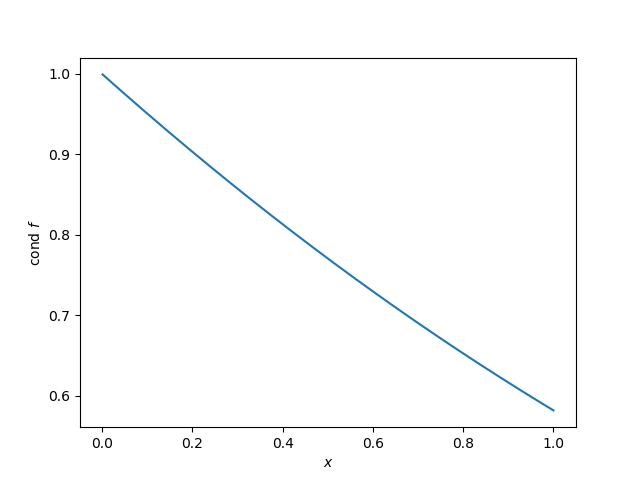
\includegraphics[width=\linewidth]{condf.png}
    \caption{$(\cond f)(x)$ on $[0, 1]$}
  \end{minipage}%
  \begin{minipage}[b]{0.5\linewidth}
    \centering
    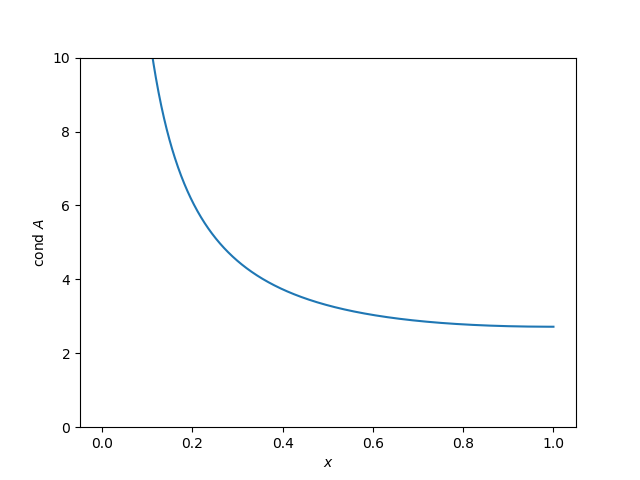
\includegraphics[width=\linewidth]{conda.png}
    \caption{$(\cond A)(x)$ on $[0, 1]$}
  \end{minipage}
\end{figure}

\textbf{(d)} $n$ bit lost when $|\Delta y / y| < 2^n \epsilon^*$, where 
$\epsilon^*$ is the floating number rounding error, while 
\begin{equation}
  \left|\frac{\Delta y}{y}\right| \approx 
  (\cond f)(x)\left[\left|\frac{x^* - x}{x}\right| + 
  (\cond A)(x^*)\epsilon\right]
  = \left(\frac{x}{\e^x-1} + \frac{\epsilon}{\epsilon^*}
    \frac{1}{1-\e^{-x}}\right)\epsilon^*
\end{equation}
Assuming $\exp$ implementation is ideal so that $\epsilon/\epsilon^* = 1$, 
$|\Delta y / y| < 2^n \epsilon^*$ gives:
\begin{equation}
  \frac{x+\e^{x}}{\e^x - 1} < 2^n
\end{equation}
\begin{itemize}
  \item For $n=1$, $x > 1.146$ meaning for all $x\in[0,1]$ there will be 
    at least 1 bit of significance lost. 
  \item For $n=2$, $x > 0.378$
  \item For $n=3$, $x > 0.152$
  \item For $n=4$, $x > 0.069$
\end{itemize}

\textbf{(e)} (d) is equivalent to requiring forward error to be 
less than $2^n\epsilon^*$. 

\textbf{(f)} for small $x$, using the series 
\begin{equation}
  f(x) = \sum_{n=1}^\infty \frac{(-x)^n}{n!}
\end{equation}
The algorithmic result:
\begin{align}
  f_A(x) &= \fl\left[\sum_{n=1}^N \frac{(-x)^n}{n!}\right] \\
         &= \sum_{n=1}^N\frac{(-x)^n}{n!}(1+n\epsilon) \\
         &= \sum_{n=1}^N\frac{(-x)^n}{n!} +
         \epsilon \sum_{n=1}^N\frac{|(-x)^n|}{(n-1)!} \\
         &= f(x) + x\e^x\epsilon + \mathcal O(x^N) 
\end{align}
With large $N$, $\mathcal O(x^N) \sim \epsilon^*$. So for $f(x_A) = f_A(x)$, 
there is: 
\begin{align}
  &x_A - x = \frac{x\e^x \epsilon}{f'} = x\e^{2x}\epsilon\\
  &(\cond A)(x) \equiv \frac{|x_A - x|}{|x|}\frac{1}{\epsilon} 
  = \e^{2x}
\end{align}
is bounded in $x\in [0,1]$ and performs better in small $x$ regime. 

\section{Limits in $\mathbb R(p,q)$}
\lstinputlisting[language=Python]{p5.py}

The above code gives output: 
\begin{lstlisting}[numbers=none]
n-stop: 10000000000000 value: 2.716110034086901
[2.         2.59374246 2.70481383 2.71692393 2.71814593 2.71826824
 2.71828047 2.71828169 2.7182818  2.71828205 2.71828205 2.71828205
 2.7185235  2.71611003]
\end{lstlisting}

(Technically it's not converged because with larger $n$ the value doesn't stop 
here but goes to $0$.)

% The sequence to converge up to $12$ significant figures means the relative 
% error is smaller than $\epsilon = 10^{-12}$. Meanwhile the sequence 
% is monotonically increasing, so for $(1+1/n)^n > \e - \epsilon$, 
% requires $n > 1.36\times 10^{12}$.
% So the minimum power-10 number is $10^{13}$

For IEEE754 double type, $q=11$, $p=52$, the rounding error $\epsilon =
2^{-52} \approx 2.22\time 10^{-16}$. The difference between $\e$ and $\e_n$
is: 
\begin{equation}
  \e - \left(1 + \frac 1b\right)^n = \frac{\e}{2n} - \frac{11\e}{24n^2} + 
  \mathcal O(n^-3) \approx \frac{\e}{2n}
\end{equation}
While the rounding error:
\begin{equation}
  \fl\left[\left(1+\frac 1n\right)^n\right] - \e_n
  \approx \left(1+\frac 1n + \epsilon\right)^n - \left(1+\frac 1n\right)^n
  \approx n\epsilon
\end{equation}
Total error $\e/2n + n\epsilon$ has minimum at $n\sim
\sqrt{e/2\epsilon} \approx 10^9$ which is consistent with the array from 
code output. However, the converge value $10^{13}$ happens in ill-behaved
regime: in Fig.(\ref{fig:p5}) we can see that the ``converged'' term $n =
10^{13}$ and $10^{14}$ locate in the oscillating area, therefore it's a
numerical coincidence. 

\begin{figure}[!htp]
  \centering
  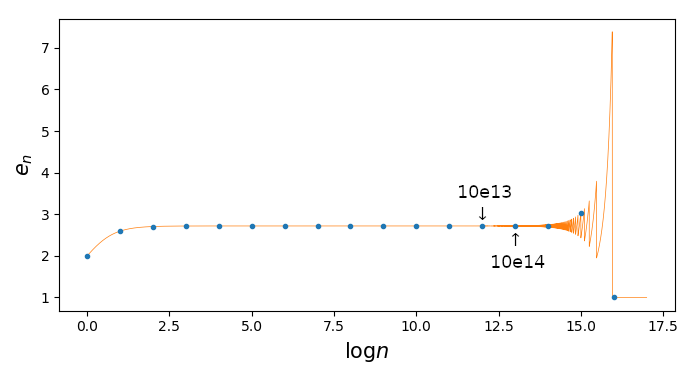
\includegraphics[width=\linewidth]{p5.png}
  \caption{$n$ series of $\e$ (log scale), orange line is continuous $n$, 
  blue dot is $n = 1, 10, 10^2, \cdots$.  The oscillation
  from right to left is $(1+k\epsilon)^n$ with $\epsilon$
  the smallest machine number step relative to $1$ and $k = 1, 2, \cdots$ 
  ($1+1/n$ is rounded to $1+k\epsilon$). \label{fig:p5}}
\end{figure}

\section{Fun with square roots}
Define $y_N\equiv x^{2^{-N}}$ meaning $N$ times square root. For $x\in [0,
1]$, $y_N = 1-k\epsilon$ where $k=0,1,2,\cdots$ and $\epsilon = 2^{-p-1}$
is the machine float number precision, i.e. rounding error
\footnote{It's $2^{-p-1}$ rather than $2^{-p}$ because $y_N < 1$ has
exponential part smaller than that of $1$ by $1$, which means that for 
machine number $1+\delta\neq 1$, smallest $\delta = 2^{-p}$ but for $1-\delta
\neq 1$, $\delta = 2^{-p-1}$. }.

Because $y_N$ is a step function of $x$, the final result $y = y_N^{2^N}$ 
is also a step function of $x$. $y=x$ only when in real calculation 
$x^{-2^{N}} = 1-k\epsilon$
(Assuming the algorithm is perfect so that the error introduced by it is
smaller than rounding error). 
\begin{figure}[!htp]
  \centering
  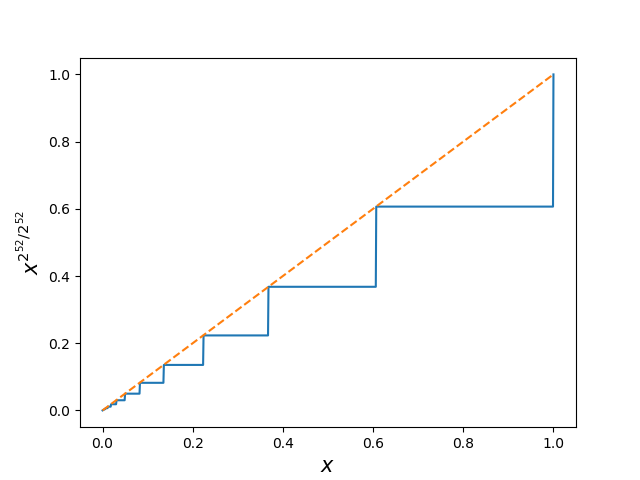
\includegraphics[width=0.8\linewidth]{p6.png}
  \caption{Square root 52 times and square 52 times}
\end{figure}

Let $M = 2^N$ and $\delta = k2^{-p-1}$, where $N$ and $p$ are close, i.e. 
$M\delta\sim 1$. The numbers that are intact are: 
\newcommand\off{{n_{\text{off}}}}
\begin{equation}
  (1-\delta)^M = \big[(1-\delta)^{1/\delta}\big]^{M\delta} \approx \e^{-M\delta}
\end{equation}
% \begin{align}
%   \left(1-\delta\right)^M 
%   &= \sum_{n=0}^M \frac{M!}{n!(M-n)!} (-\delta)^n \\
%   &= \sum_{n=0}^{\off} \frac{\sqrt{2\pi M}(M/\e)^M}{n!\sqrt{2\pi(M-n)}
%   \big[(M-n)/e\big]^{M-n}} (-\delta)^n
%   + \mathcal O\left(\frac{(M\delta)^{\off}}{\off!}\right)
%   \label{eq:stiring} \\
%   &=\sum_{n=0}^{\off} \frac{(-M\delta)^n}{n!\e^{-n}}
%   \left(1-\frac{n}{M}\right)^{n-1/2} \left(1-\frac{n}{M}\right)^M
%   + \mathcal O\left(\frac{(M\delta)^{\off}}{\off!}\right) \\
%   &\approx \sum_n^\off\frac{(-M\delta)^n}{n!\e^{-n}}\e^{-n}
%   = \e^{-M\delta} + \mathcal O\left(\frac{(M\delta)^{\off}}{\off!}\right)
%   \approx \e^{-M\delta}
% \end{align}
% where Eq.~(\ref{eq:stiring}) applies Stirling formula and the remaining term
% is bounded for $1 \ll \off \ll M$. 

Plug $M$ and $\delta$ in, the intact numbers are $\{\exp[-k
2^{N-p-1}]: k = 0, 1, 2, \cdots\}$.
Specifically for double precision $p = N = 52$, they are $\{1, \sqrt \e, 
  \e^{-1}, \e^{-1.5}, \cdots\}$. This result is validated in
  Fig.~(\ref{fig:p6_val})

\begin{figure}[!htp]
  \begin{minipage}[b]{0.5\linewidth}
    \centering
    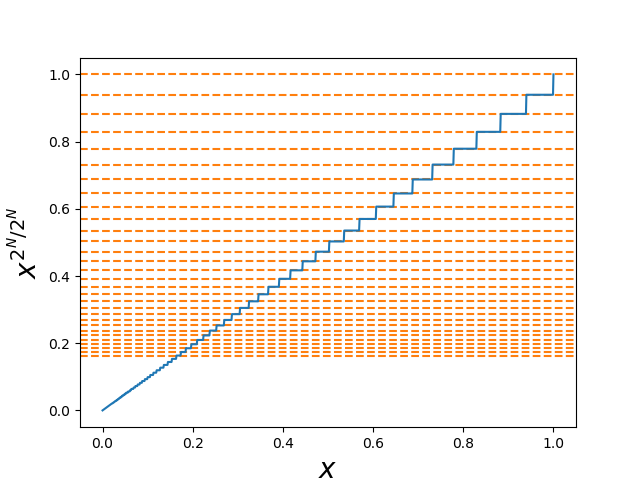
\includegraphics[width=\linewidth]{p6_49.png}
  \end{minipage}%
  \begin{minipage}[b]{0.5\linewidth}
    \centering
    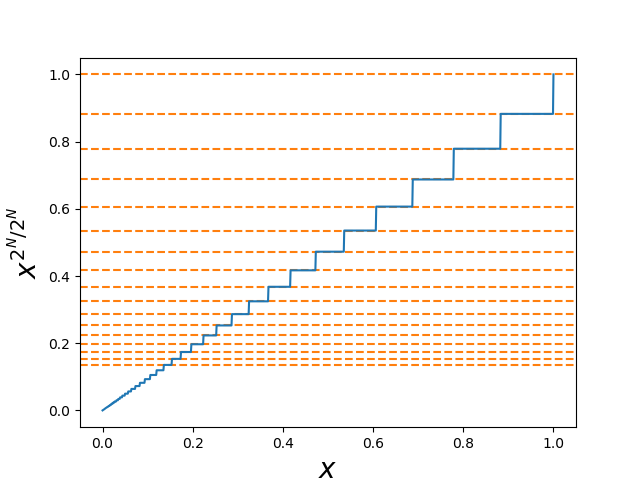
\includegraphics[width=\linewidth]{p6_50.png}
  \end{minipage}\\
  \begin{minipage}[b]{0.5\linewidth}
    \centering
    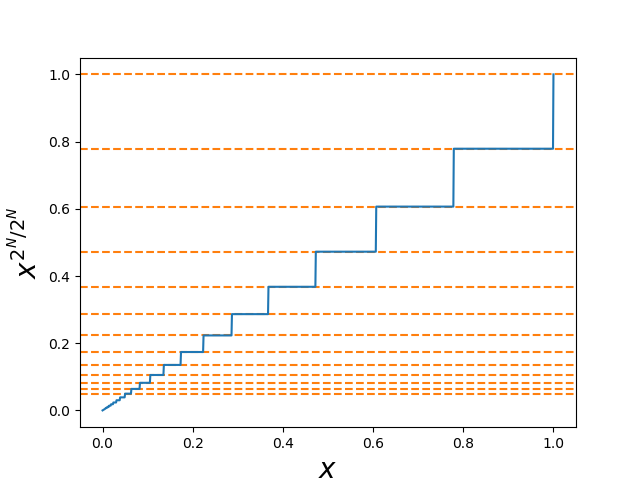
\includegraphics[width=\linewidth]{p6_51.png}
  \end{minipage}%
  \begin{minipage}[b]{0.5\linewidth}
    \centering
    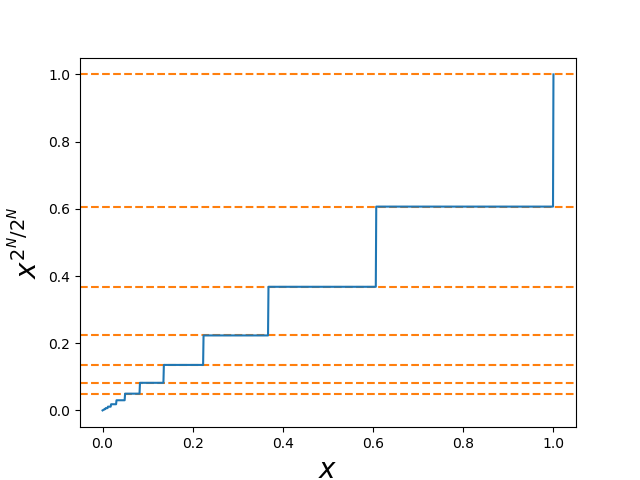
\includegraphics[width=\linewidth]{p6_52.png}
  \end{minipage}\\
  \begin{minipage}[b]{0.5\linewidth}
    \centering
    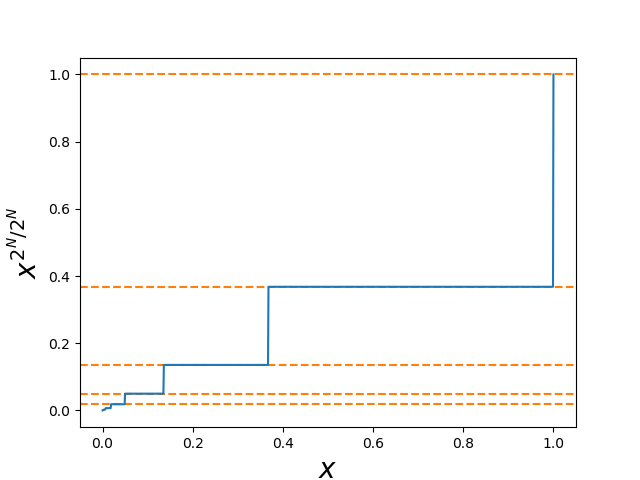
\includegraphics[width=\linewidth]{p6_53.png}
  \end{minipage}%
  \begin{minipage}[b]{0.5\linewidth}
    \centering
    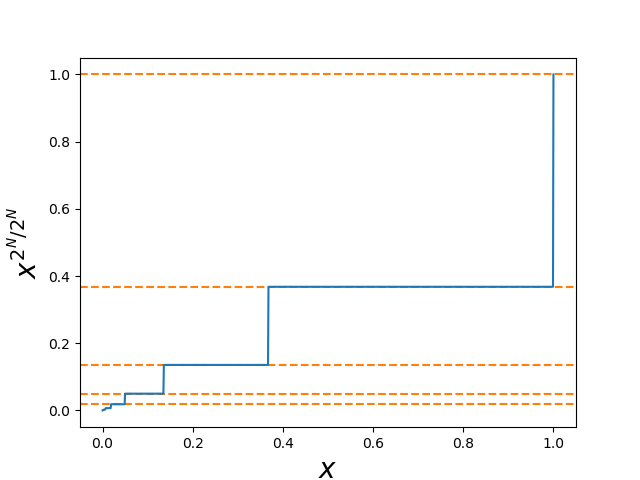
\includegraphics[width=\linewidth]{p6_54.png}
  \end{minipage}
  \caption{Validation of problem 6 with $N = 49, 50, 51, 52, 53, 54$
  respectively. Horizontal line is $\{\exp[-k2^{N-53}]: k\in\mathbb N\}$. 
\label{fig:p6_val}} 
\end{figure}

\section{The issue with polynomial roots}
For $N = 20$
\begin{equation}
  a_n = (-)^{N-n}\sum_{|\{p\}|=n} \prod^N_{k\notin \{p\}} k
  = (-)^{N-n}\sum_{1\le q_0 < q_1 < \cdots < q_{N-n} \le N}
  \prod_i q_i
\end{equation}

\textbf{(a)} This is calculated by the following script: 
\lstinputlisting[language=Python, lastline=17]{p7.py}
The result is (from $a_{20}$ to $a_{0}$):
\begin{lstlisting}[numbers=none]
[1 -210 20615 -1256850 53327946 -1672280820 40171771630 -756111184500
 11310276995381 -135585182899530 1307535010540395 -10142299865511450
 63030812099294896 -311333643161390640 1206647803780373360
 -3599979517947607200 8037811822645051776 -12870931245150988800
 13803759753640704000 -8752948036761600000 2432902008176640000]
\end{lstlisting}

\textbf{(b)} The polynomial is already bad behaved in evaluation using 
double precision. 
\lstinputlisting[language=Python, firstline=19, firstnumber=18, lastline=23]{p7.py}
This script shows that for integer (perfect precision in Python) the
polynomial behaves as we expect (all 0s) 
but for float evaluation it deviates. 

\lstinputlisting[language=Python, firstline=24, firstnumber=23, lastline=33]{p7.py}
The Newton's method \texttt{scipy.iptimize.root} finds the root near 21 to 
be 19.9999717. 

\textbf{(c)} for $\delta = 10^{-8}, 10^{-6}, 10^{-4}, 10^{-2}$, 
the root finder gives root to be 9.58534944, 7.75272109, 5.9693346,
5.46959278 respectively.
\lstinputlisting[language=Python, firstline=34, firstnumber=33, lastline=37]{p7.py}

\textbf{(d)} The root finder converges to the same roots about 8.92 
(from function evaluation we can see more digits are not meaningful). 
\lstinputlisting[language=Python, firstline=38, firstnumber=37, lastline=43]{p7.py}

Companion matrix eigenvalue algorithm shows that there's no real roots 
between 10 and 20. 

\textbf{(e)} For a differentiate $\dif \vec a$, there is: 
\begin{align}
  &p(\Omega_k + \dif\Omega_k) + \sum_\ell \Omega_k^\ell \dif a_\ell = 0 \\
  \Rightarrow &
  \dif\Omega_k = -\sum_\ell \frac{\Omega_k^\ell}{p'(\Omega_k)} \dif a_\ell \\
  \Rightarrow &
  \frac{\partial\Omega_k}{\partial a_\ell} =
  -\frac{\Omega_k^\ell}{p'(\Omega_k)}
\end{align}
So for condition number: 
\begin{equation}
  (\cond \Omega_k)(\vec a) \equiv \sum_\ell \Gamma_{k\ell} 
  \equiv \sum_\ell \left|\frac{\partial\Omega_k}{\partial a_\ell}
  \frac{a_\ell}{\Omega_k}\right| 
  =\sum_\ell \frac{\Omega_k^{\ell-1}|a_\ell|}{|p'(\Omega_k)|}
  \label{eq:condOmega}
\end{equation}

For $\Omega_k = 14, 16, 17, 20$, Eq.~(\ref{eq:condOmega}) evaluates to
5.4e13, 3.5e13, 1.8e13 and 1.4e11 respectively. These results are
significantly larger than 1, which means that small difference in $\vec a$ 
can change roots unbounded. 

No algorithm can help us because this is intrinsic to the problem. Any
algorithm that reflects the problem faithfully cannot decrease the
conditioning number of the problem itself. 
This suggests that using coefficients for polynomial with high degree 
is an ill-behaved problem and should be avoided. 

\section{Recurrence in reverse}
(i) $0 < y_{n+1} $, so $y_n < \e/(n+1)$.
Similarly $y_{n+1} < e/(n+2)$, which means $\e/(n+2) < y_n < \e/(n+1)$, 
so $y_{n+1}/y_n < 1$, and with large $n$, this ratio goes to $1$. 
Using this bounded approximation for $y_n$, 
error from $y_{n+1}$ to $y_n$ is (assuming $n$ as an integer is perfect
machine number, neglect error in $\e$): 
\begin{align}
  y_n = \frac{\e - y_{n+1}}{n+1}
  \quad\Rightarrow\quad
  \frac{\Delta y_n}{y_n} 
  &= \frac{1}{n+1}\frac{\Delta y_{n+1}}{y_n} + \epsilon_\div 
  = \frac{1}{n+1} \frac{y_{n+1}}{y_n} \frac{\Delta y_{n+1}}{y_{n+1}}
  + \epsilon_\div \\
  &< \frac{1}{n+1}\frac{\Delta y_{n+1}}{y_{n+1}} + \epsilon_\div 
\end{align}
So for a large $N$ and reversed recurrence result $y_k$ with $k<N$, 
\begin{align}
  \frac{\Delta y_k}{y_k} 
  &<
  \frac{k!}{N!}\delta_N + \sum_{i=0}^{N-k} \frac{k!}{(N-i)!} \epsilon_\div \\
  &\lesssim \frac{k!}{N!}\delta_N + \epsilon_\div
  \label{eq:deltay}
\end{align}
where $\delta_N = \Delta y_N / y_N$
is the error in $y_N$ and the last step is estimated for 
large $N$ and $k$. Given tolerance $\epsilon$, 
\begin{itemize}
  \item $\epsilon$ cannot be smaller than rounding error when do division 
    $\epsilon_\div$
  \item With larger $N$, error introduced from $y_N$ will vanish. 
  \item $N-k\sim \log_k[(\epsilon - \epsilon_\div)/\delta_N]$
    will be good enough for $y_k$ with tolerance $\epsilon$
\end{itemize}

(ii) Since $\delta_N$ influence goes to $0$ with large $N$, we don't need precise 
$y_N$ for the algorithm. We can choose $y_N \approx e/(N+1)$ as the initial 
number for a big $N$. 

\textbf{(a)} From Eq.(\ref{eq:deltay}), with $\epsilon_\div = 0$
the condition number is: 
\begin{equation}
  (\cond g_k)(y_N) = \left|\frac{\Delta y_k / y_k}{\Delta y_N / y_N}\right|
  \lesssim \frac{k!}{N!}
\end{equation}

The expression becomes $\cond g_k = k!/N!$ when $N$ is large. 

\textbf{(b)} This means $\epsilon \lesssim k!/N!$ or $N >
\Gamma^{-1}(k!\epsilon^{-1})$. A very loose approximation
is $N > k + \log_k \epsilon$. 

\textbf{(c)} For IEEE754 double type, $\epsilon = \text{eps} = 2^{-52}$, 
for $k = 21$, $N > 31$

\textbf{(c)} Note that for $N=32$, output for error is 0. 
\lstinputlisting[language=Python]{p8c.py}

\end{document}
% vim: ts=4 sw=2 sts=4 expandtab
